\subsection{Actors}
In the model several actors are defined, with different functionalities.
\begin{itemize}
    \item \textbf{Entity}: Company or organization (legal person). An entity can be one or both:
          \begin{itemize}
              \item \textbf{Service Provider}: Entity which requests information from a subject, so \textbf{it creates Presentation Requests and receives Presentations}.
              \item \textbf{Issuer}: It can help anyone to create a new identity. Also this kind of entity can emits certified information about a subject, so \textbf{it creates Credentials}.
          \end{itemize}
    \item \textbf{Subject}: Person (natural or legal) who \textbf{has information certified by an Issuer and sends it to a Service Provider}, so it receives credentials and creates presentations. It is the information owner. This information is saved and controlled from a wallet.
    \item \textbf{Admin}: It is the \textbf{identity} (account) \textbf{that deployed the Smart Contracts}. \textbf{It is only used to create the first entity} (Issuer). \textbf{All other identities must be created by Issuers}.
\end{itemize}
In the next figure (\ref{fig:roles-ala}) we can see a visual explanation of the data flow between the different actors.
\begin{figure}[h]
    \centering
    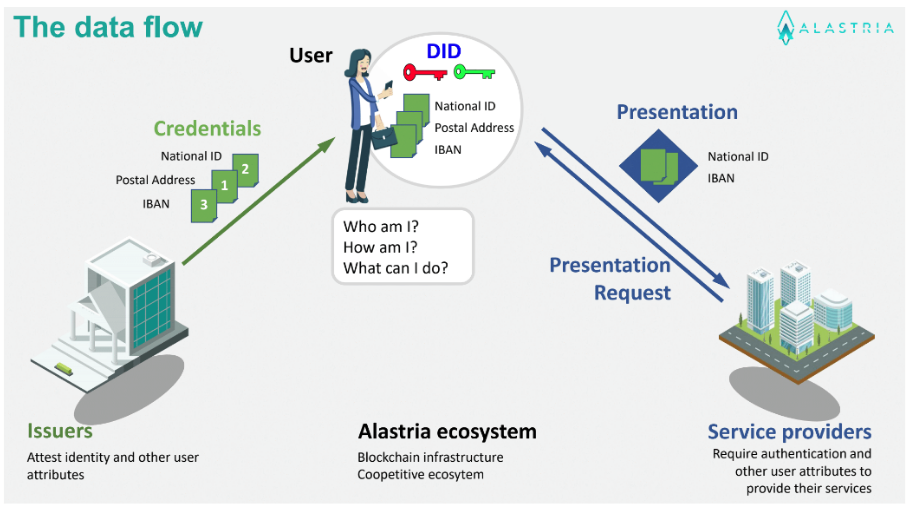
\includegraphics[width=1.0\textwidth]{images/Alastria ID/roles-ala.png}
    \caption{Data flow between different actors in Alastria}
    \label{fig:roles-ala}
\end{figure}
